% 0594(본책 106쪽) — 지름 BD 인 원 O, 접선 EC(접점 C), AD∥EC, AC·BD 의 교점 P, ∠BCE=28°, ∠APD 표시. 스캔 삽화를 TikZ 로 다시 그림.
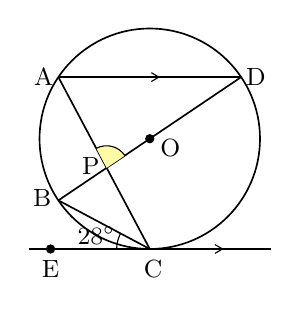
\begin{tikzpicture}[scale=1.4, line width=0.6pt]
  \draw (0.000,0.000) circle (1.000);
  \draw (-1.100,-1.000) -- (1.100,-1.000);
  \draw (-0.829,0.559) -- (0.829,0.559);
  \draw (-0.829,0.559) -- (-0.000,-1.000);
  \draw (-0.829,-0.559) -- (0.829,0.559);
  \draw (-0.829,-0.559) -- (-0.000,-1.000);
  \fill (0.000,0.000) circle (1.2pt);
  \fill (-0.900,-1.000) circle (1.2pt);
  \draw[line width=0.4pt] (0.014,0.519) -- (0.083,0.559) -- (0.014,0.599);
  \draw[line width=0.4pt] (0.591,-1.040) -- (0.660,-1.000) -- (0.591,-0.960);
  \draw[line width=0.4pt] (-0.265,-0.859) arc[start angle=152.000, end angle=180.000, radius=0.300];
  \node[font=\small, inner sep=1pt] at (-0.485,-0.879) {$28^\circ$};
  \fill[yellow!35] (-0.391,-0.264) -- ++(34.000:0.200) arc[start angle=34.000, end angle=118.000, radius=0.200] -- cycle;
  \draw[line width=0.4pt] (-0.226,-0.152) arc[start angle=34.000, end angle=118.000, radius=0.200];
  \node[font=\small, anchor=west, inner sep=1.5pt] at (0.050,-0.080) {O};
  \node[font=\small, anchor=east, inner sep=1.5pt] at (-0.829,0.559) {A};
  \node[font=\small, anchor=west, inner sep=1.5pt] at (0.829,0.559) {D};
  \node[font=\small, anchor=east, inner sep=1.5pt] at (-0.849,-0.539) {B};
  \node[font=\small, anchor=north, inner sep=1.5pt] at (0.030,-1.060) {C};
  \node[font=\small, anchor=north, inner sep=1.5pt] at (-0.900,-1.060) {E};
  \node[font=\small, anchor=east, inner sep=1.5pt] at (-0.411,-0.244) {P};
\end{tikzpicture}
